\chapter{Аналитический раздел}
\label{cha:analysis}
В данном разделе приведены основные сведения о размытие движения, о методах и алгоритмах его программной генерации.

\section{Природа размытия движения}

\subsection{Причины появления смаза}

Причины возникновения размытия изображений при съёмке камерой связаны со способом захвата изображения. Свет попадает на светочувствительную матрицу устройства. Затвор и диафрагма влияют на количество света, попавшего на матрицу. Затвор ограничивает время, в течение которого свет попадает на матрицу и формируется итоговое изображение. Данное время называется выдержкой.
\par
После открытия затвора матрица начинает аккумулировать весь свет, попавший на неё. Так как во время движения объекта отраженные лучи света меняют своё положения, то во время выдержки все проекции объекта на плоскость матрицы будут запечатлены на итоговом изображении.
\par
Данный процесс выдержки может быть формализован с помощью уравнения \eqref{F:F2_1_1} . Во время съемки сцены,  представляет собой содержимое плоскости изображения. Захваченный свет является результатом аккумулирования входящего излучения $L$ в течение времени выдержки $\Delta T$. Функция $f$ моделирует влияние оптики, затвора, диафрагмы, светочувствительности матрицы.
\par
\begin{eqndesc}
    \begin{equation}
        I = \int_{\Delta T} f(t) \cdot L(t) dt
        \label{F:F2_1_1}
    \end{equation}
    , где 
    $I$ "--- выходная интенсивность изображения;\\        
    $\Delta T$ "--- время выдержки;\\        
    $L(t)$ "--- входящее излучение на матрицы;\\        
    $f(t)$ "--- влияние оптики, затвора и прочих физических характеристик захвата излучения.        
\end{eqndesc}
\par
Уравнение \eqref{F:F2_1_1} дает представления о характеристиках получаемых изображений  \cite{Navarro11}. Можно сказать, что финальное изображения состоит из объединения моментальных снимков. Моментальный снимок - это снимок с временем выдержки, стремящемся к нулю.

\subsection{Описание характеристик смаза}
\label{cha:analysis_charestic}
Для изображения кадра перемещения сферы радиуса, соизмеримого с одним пикселем, необходимо отобразить путь пройденный этой сферой за время выдержки $\Delta T$. Так как любой объект можно представить в виде набора точек, то конечное изображение будет иметь вид следа перемещения объекта за время выдержки.
\par
Для упрощения задачи характеристики смаза, кривую перемещения любого тела можно представить в виде ломанной линии, где каждая точка ломанной есть точка времени начала/окончания выдержки. Такое упрощение возможно, так как время выдержки обычно равно периоду обновления экрана (При частоте обновления кадра 25 Гц выдержка равна 40 мс). Тогда любой путь объекта во время выдержки будет его перемещением. Для единичного пикселя смаз будет представлять собой отрезок, соединяющий точки нахождения пикселя в моменты времени начала и окончания выдержки.
\par
Из выше указанных замечаний можно выдвинуть следующие требования для генерации смазывания движущихся объектов:
\begin{enumerate}
    \item Смаз содержит изображения объекта в моменты времени начала и окончания выдержки;
    \item Смазывание формируется вдоль вектора движения объекта;
    \item Продолжительность смаза зависит от скорости движения объекта;
    \item Объекты без движения не подвергаются смазыванию;
    \item Смаз не терпит разрывов;
    \item Интенсивность изображения без движения соизмерима с интенсивностью смазанного изображения.
\end{enumerate}

\section{Методы размытия движения}

\subsection{Размытие движения с помощью накопительного буфера}
\label{cha:analysis_acum}

Одним из первых решений, которое было предложено - это склеивание нескольких отрендеренных изображений   \cite{Haeberli90}. Заметим, что интенсивность изображения должна быть соизмерима с начальной. С учетом данного утверждения получим формулу \eqref{F:F202}.
\begin{eqndesc}
    \begin{equation}\label{F:F202}
        I(t, \Delta T, N) = \frac{ \sum_{i=0}^{N} { V({t - \frac{i}{N} \cdot \Delta T})}}{N}
    \end{equation}
    \\
    где $t$ "--- время окончания выдержки \\
    $\Delta T$ "--- продолжительность выдержки \\
    $V(t)$ "--- мгновенный снимок в момент времени $t$\\
    $N$ "--- количество мгновенных снимков \\
    $I(t, \Delta T, N)$ "--- изображение с выдержкой $\Delta T$
\end{eqndesc}

Для достижения наивысшей скорости отрисовки изображения при генерации видео ряда необходимо накапливать результаты генерации последних $N$ моментальных снимков в буфере. Постоянность выдержки $\Delta T$ и частоты обновления экрана $fps$  позволяет на каждой итерации отрисовать следующее количество новых кадров  $k = \frac{N}{fps \cdot \Delta T}$, $k \in Z$
\par
Очевидно, что достигается максимальная скорость работы алгоритма при $k = 1$, т.е. когда $fps = \frac{N}{\Delta T}$


\begin{table}[ht]
    \caption{Зависимость частоты кадров от количества мгновенных снимков и времени выдержки}
    \begin{tabular}{|c|r|r|r|r|}
        \hline
        $\Delta T$, c & $N =8$ & $=16$ & $=32$ & $=64$ \\
        \hline
        $1$           & 8      & 16    & 32    & 64    \\
        $\frc{1}{2}$  & 16     & 32    & 64    & 128   \\
        $\frc{1}{4}$  & 32     & 64    & 128   & 256   \\
        $\frc{1}{8}$  & 64     & 128   & 256   & 512   \\
        $\frc{1}{16}$ & 128    & 256   & 512   & 1024  \\
        \hline
    \end{tabular}
    \label{tab:acum_table}
\end{table}

Проанализировав зависимость частоты кадров от количества мгновенных снимков и времени выдержки (таблица \ref{tab:acum_table}), можно прийти к следующему выводу. Чтобы получить изображение с малой выдержкой при большом количестве семплов нужно иметь большую частоту генерации кадров, что становится преградой для реализации размытия в режиме реального времени данным методом.

\subsection{Размытие движения с помощью скорости пикселя}
\label{cha:analysis_pixelblur}


В пункте \ref{cha:analysis_charestic} были сделаны предположения о природе смаза. Если рассматривать каждый пиксель изображения за время выдержки, то можно восстановить путь пройденный каждым пикселем с помощью мгновенной скорости каждого пикселя в момент начала/окончания выдержки.


\par
Для реализации такого размытия можно использовать следующую идею. Цвет каждого пикселя размытого изображения представить, как среднее арифметическое цветов пикселей вдоль вектора направления скорости вычисляемого пикселя   \cite{GpuGems2008}. Данная идея представлена в формуле \eqref{F:F2_2_1}. 

\begin{eqndesc}
    \begin{equation}\label{F:F2_2_1}
        I(x,y) = \frac{\sum_{i=0}^{N} {V(x + i \cdot v_x, y + i \cdot v_y)}}{N}
    \end{equation}
    \\
    где $x,y$ "--- координаты пикселя \\
    $v$ "--- мгновенная скорость размываемого пикселя  \\
    $V(x,y)$ "--- цвет пикселя мгновенного снимка \\
    $I(x,y)$ "--- цвет размытого пикселя
\end{eqndesc}



Данный подход позволяет генерировать размытие по одному снимку. Данный способ намного быстрее предыдущего, но обладает не идеальными графическими параметрами (рисунок \ref{fig:pixel_blur}).


\begin{figure}[h]
    \centering
    \begin{minipage}[h]{0.49\linewidth}
        \center{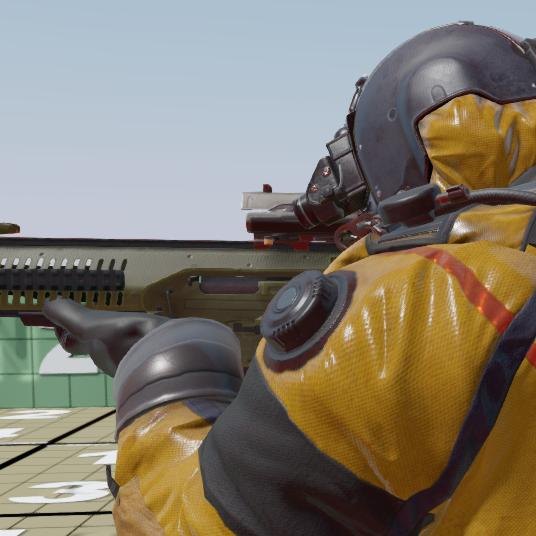
\includegraphics[width=0.5\linewidth]{img/blur_1.jpg} \\ а)}
    \end{minipage}
    \hfill
    \begin{minipage}[h]{0.49\linewidth}
        \center{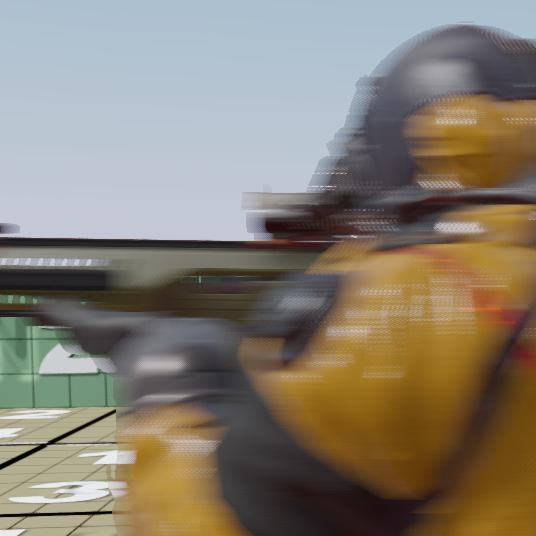
\includegraphics[width=0.5\linewidth]{img/blur_2.jpg} \\ б)}
    \end{minipage}
    \caption{Сравнение смаза. \\ а) Исходное изображение б) Изображение с размытием по скорости пикселя}
    \label{fig:pixel_blur}
\end{figure} 

\par
Данный метод оставляет резкую границу раздела заднего плана и смазываемого изображения. Это происходит из-за резкого перепада скорости фона и движущегося тела. Также при перекрытии движущегося тела статическим образуются артефакты отрисовки на границе тел. Неподвижное тело не смазывается, но на границе тел скорость резко меняет свое значение, и в соответствии с формулой \eqref{F:F2_2_1} интенсивность пикселя будет составляться и из части изображения неподвижного тела.
\par
Из выше сказанных слов делаем вывод, что данный метод смазывания работает без видимых артефактов  при равномерно-распределенной скорости каждого пикселя, например, при смене ракурса камеры.

\subsection{Размытие движения с помощью максимальной скорости движения участка изображения и буфера глубины}
\label{cha:analysis_mcgiure}

Проблему резких границ размытия было предложено решать с помощью снижения размерности буфера скоростей и анализа соседних участков буфера. Изображение разбивается на участки размера $k \times k$ пикселей, и для каждого участка ищется максимальная скорость. Такое преобразование из буфера скоростей пикселей можно сделать по формуле \eqref{F:F2_3_1}.
\begin{eqndesc}
    \begin{equation}\label{F:F2_3_1}
        TileMax[x,y] = \max_{u \in [o ; k)} {
        \max_{v \in [o ; k)} {v [kx + u; ky + v]}
        }
    \end{equation}
    , где $\max$ "--- максимальный вектор по длине; \\
    $v$ "---  буфер скоростей;\\
    $k$ "---  размерность участка.

\end{eqndesc}

Чтобы проанализировать все пиксели, которые вносят вклад в размытие того или иного пикселя необходимо, чтобы $|v[x,y]| \le k $ \space $\forall x,y $. Следующим шагом предлагается найти доминирующую скорость для соседей участка и самого участка.


Использование буфера максимальной скорости движения участков, задаваемого уравнение \eqref{F:F2_3_2}, решает проблему резких границ размытия.

\begin{eqndesc}
    \begin{equation}\label{F:F2_3_2}
        NeighborMax[x,y] = \max_{u \in [-1 ; 1]} {
            \max_{v \in [-1 ;1]} {TileMax [x + u; y + v]}
        }
    \end{equation}
    , где $\max$ "--- максимальный вектор по длине; \\
    $TileMax$ "---  буфер максимальных скоростей участков по формуле \eqref{F:F2_3_1}.
\end{eqndesc}

В методе размытия с помощью скорости пикселя суммировался цвет всех пикселей, даже тех, которые не являлись частью смаза текущего объекта. Чтобы решить данную проблему, было предложено при расчете каждого пикселя $A$ анализировать вклад $\alpha_i$ для каждого соседнего пикселя $B_i$ вдоль  вектора скорости $NeighborMax[\frac{A_x}{k}, \frac{A_y}{k}]$. Морган Макгуайр предложил считать, что пиксель $B_i$ вносит вклад $\alpha_i$ в смаз пикселя $A$ при следующих условиях:
\begin{enumerate}
    \item Условия вклада переднего плана
          \begin{enumerate}
              \item пиксель $B_i$ ближе к наблюдателю чем $A$
              \item пиксель $A$ находится в пределах разброса точек $B_i$;
          \end{enumerate}
    \item Условия вклада фона
          \begin{enumerate}
              \item пиксель $B_i$ дальше от наблюдателя чем $A$
              \item $B_i$ находится в пределах разброса точек $A$
          \end{enumerate}
    \item Условие для единого тела
          \begin{enumerate}
              \item пиксели $A$ и $B_i$ находятся в пределах разброса точек друг друга;
          \end{enumerate}
\end{enumerate}


Разбросом точек пикселя называем окружность с центром в данном пикселе и радиусом скорости данного пикселя. Было предложено вклад пикселя считать по формуле \eqref{f:f20_pertileblur} и интенсивность пикселей считать по формуле \eqref{f:f20_pertileblur_I}.
\begin{eqndesc}
    \begin{eqnarray}
        \label{f:f20_pertileblur}
        \alpha_i =
        depthCompare(Z[A], Z[B_i]) \cdot cone(B_i, A, v_{B_i}) + \\
        + depthCompare(Z[B_i], Z[A]) \cdot coe(A, B_i, v_A) + \\
        + cylinder(B,A,v_{B_i}) \cdot cylinder(A,B, v_A) \cdot 2
    \end{eqnarray}
    ,где
    $Z$ "--- буфер глубины; \\
    $A$ "--- координаты анализируемого пикселя; \\
    $B_i$ "--- соседний пиксель пикселя $A$ вдоль вектора скорости; \\ 
    $v_A$ "--- скорость пикселя $A$; \\
    $v_{B_i}$ "--- скорость пикселя $B_i$. \\

\end{eqndesc}
\par 

\begin{eqndesc}
    \begin{equation} \label{f:f20_pertileblur_I}
        I(A) = \frac{\frac{V[A]}{|v_A|} +
        \sum_{i=1}^N
        {\alpha_i \cdot V[A + v_A \cdot i]}
        }{\frac{1}{|v_A|} + \sum_{i=1}^N  a_i}
    \end{equation}
    , где  $V$ "--- буфер кадра;\\
    $\alpha_i$ "--- вклад пикселя по формуле \eqref{f:f20_pertileblur};\\
    $N$ "--- количество проходов;\\
    $v_A$ "--- скорость пикселя $A$; \\
    $I(A)$ "--- интенсивность пикселя $A$ с учетом смаза
\end{eqndesc}

Описание вспомогательных функций:
\begin{itemize}
    \item $clamp(x, L, R) = min(R, max(L, x))$ - ограничение диапазона значений $x$ отрезком $[L;R]$
    \item $depthCompare(z_A, z_B) = clamp(1 - \frac{z_A - z_B}{EXTENT}, 0, 1)$ - проверка отдаленности точки $B$ по стравнению с точкой $A$. $EXTENT$ - константа достаточного расстояния между точками. Обычно константа берется от 1 мм до 10 см  \cite{McGuire12}.
    \item $cone(v, A, B) = clamp(1 - \frac{|A-B|}{|v|}, 0,1)$ - проверка на вхождение точки $B$ в разброс точек точки $A$
    \item $smoothstep(x) = 3 t^2 - 2t^3$, где $t = clamp(x, 0, 1)$ -  проверка принадлежности $x$ краям отрезка $[0, 1]$
    \item $smoothstep(x, L, R) = smoothstep(\frac{x - L}{R -
                  L})$ - проверка принадлежности $x$ краям отрезка $[L; R]$
    \item $cilinder(v, A, B) = 1 - smoothstep(0.95 |v|, 1.05|v|, |A - B|)$ - проверка на присутствие точки $B$ на границе разброса точек точки $A$ со скоростью $v$
\end{itemize}

Такой метод выполняет смазывания за три прохода по плоскости изображения и требует в качестве входных данных буферы глубины и скоростей пикселей. Данный метод может применяться для генерации изображение в реальном времени. Данный метод может работать с резкими перепадами значений буферов.

\subsection{Сравнение методов размытия движения}

В пунктах \ref{cha:analysis_acum}, \ref{cha:analysis_pixelblur}, \ref{cha:analysis_mcgiure} были приведены основные сведения о методах генерации размытия движения.
\par

Метод размытия движения с помощью накопительного буфера показывает наиболее близкое к природе решение, но имеет большую вычислительную сложность, что делает его не целесообразным при генерации видео-потока в режиме реального времени, но можно использовать для генерации фотоизображений.
\par
Метод размытия движения с помощью скорости пикселя рассчитан на работу с маленькой выдержкой, что позволяет грубо апроксимировать перемещение всех пикселей изображения. Алгоритм работает за один проход по плоскости изображения, что позволяет его использовать для работы в режиме реального времени. Но для размытия движения объекта могут появляться графические артефакты. При размытии движения камеры при статической сцене - артефакты не проявляются.
\par
Метод размытия движения с помощью максимальной скорости движения участка изображения и буфера глубины является модификацией предыдущего метода с устранением проблем резких границ смаза и артефактов смаза статического переднего плана.

На основании выше указанных фактов в таблице \ref{tab:compare_smooth} представлено сравнение методов генерации размытия движения.
\begin{center}
    \begin{longtable}{|p{0.2\textwidth}|p{0.2\textwidth}|p{0.2\textwidth}|p{0.30\textwidth}|}

        \caption{Сравнение методов генерации размытия движения}
        \label{tab:compare_smooth}
        \\ \hline
        Метод размытия движения                                            & с помощью накопительного буфера & с помощью скорости пикселя & с помощью максимальной скорости движения участка изображения и буфера глубины \\
        \hline \endfirsthead
        \subcaption{Продолжение таблицы~\ref{tab:compare_smooth}}
        \\ \hline \endhead
        \hline \subcaption{Продолжение на след. стр.}
        \endfoot
        \hline \endlastfoot
        Генерация изображения с большой выдержкой                          & +                               & -                          & -                                                                             \\
        \hline
        Генерация изображения с малой выдержкой                            & +                               & +                          & +                                                                             \\
        \hline
        Генерация изображения в режиме реального времени выдержкой         & Только при большой выдержке                               & +                          & +                                                                             \\
        \hline
        Генерация смаза движения перекрывающихся объектов разных скоростей & +                               & С видимыми артефактами                          & +                                                                             \\
    \end{longtable}
\end{center}


Из сравнения методов можно сделать вывод, что каждый находит свое применение при тех или иных задачах. Принято решено реализовать три метода и сравнить их характеристики в следующих задачах:
\begin{itemize}
    \item Генерация единичных фотоизображений с размытием движения
    \item Генерация анимации движения камеры с размытием
    \item Генерация анимации движения тел со статической камерой
\end{itemize}

\par
Для реализации данных методов необходимо предварительная подготовка следующих данных:
\begin{itemize}
    \item Несмазанное изображение или серия изображений
    \item Буфер глубины (z буфер)
    \item Буфер скоростей пикселей  
\end{itemize}
\par 
С учетом данных требований будет проведен следующий анализ алгоритмов удаления невидимых линий и поверхностей.


\section{Удаление невидимых линий и поверхностей}

Данные алгоритмы разработаны, чтобы показывать пользователю только те поверхности и ребра, которые находятся в поле зрения наблюдателя. Данная задача является необходимой, чтобы устранить неоднозначность отображения трехмерной модели.

\subsection{Алгоритм плавающего горизонта}

Алгоритм плавающего горизонта применяется для удаления невидимых линий при изображении трехмерных плоскостей, задаваемых функциями вида $F(x,y,z) = 0$  \cite[c. 233]{Rogers89}. 
\par
Идея алгоритма заключается в анализе пересечения данной функции с режущими плоскостями вида $z = const$. Пересечения, представляющие собой кривые, рассматриваются в порядке удаления от наблюдателя. Для каждой режущей плоскости для определенного значения $x$  и соответствующего значения $y$ кривой сравнивается со значениями $y$ для всех предыдущих кривых при том же значении $x$. Если точка выше или ниже всех других точек, тогда она видима. Таким образом алгоритм работает в пространстве изображения.
\par
Данный алгоритм можно модифицировать для построения полигональных моделей, но тогда будет требоваться строгая сортировка полигонов по удалению от наблюдателя, что не в каждой сцене достижимо.

\subsection{Алгоритм Робертса}

Робертсу удалось одним из первых решить проблему удаления невидимых линий и поверхностей. Данный алгоритм работает в пространстве объектов сцены. Алгоритм удаляет в первую очередь нелицевые грани тел. Затем удаляются перекрытия одних тел другими  \cite[с. 250]{Rogers89}.

\par
Данный алгоритм работает с объектами как с набором пересекающих плоскостей, из-за чего возможна работа только с выпуклыми телами. Для построения полигональных моделей, необходимо предварительное разбиение тел на выпуклые тела.
\par
Идеей первого этапа является анализ по какую сторону от плоскости находится наблюдатель, если наблюдатель находится по отрицательную сторону плоскости, то грань, образуемая этой плоскостью невидима.
\par
Затем требуется найти отрезки, которые перекрываются другими телами. Для этого каждое остававшееся ребро необходимо сравнить с другими телами сцены. Для ускорения процесса рекомендуется отсортировать ребра по удалению от наблюдателя.

\subsection{Алгоритм Варнока}

Алгоритм Варнока работает по принципу "разделяй и властвуй".  Алгоритм работает в пространстве изображения, которое разбивается на окна, пока задача по определению, какой сегмент нужно отрисовать в данном окне, не станет тривиальной. Таким образом разбиение изображение возможно до одного пикселя  \cite[с. 290]{Rogers89}. 
\par
Варнок изначально предложил делить окна на одинаковые четыре подокна, но данный алгоритм варьируется способами разбиения изображения на подокна. Например, Вейлером и Азертоном было предложено разбивать окна по границам многоугольников.
\par
Данный алгоритм хорошо работает для простых сцен с малым количеством тел. Но с ростом сложности сцены разбиваться сцена может вплоть до одного пикселя, что плохо сказывается на производительности.

\subsection{Алгоритм, использующий список приоритетов}

Для работы данного алгоритма необходимо предварительно отсортировать по глубине грани тел. Так как элементы, расположенные ближе к наблюдателю, перекрывают элементы, находящиеся за ним, проблема удаления невидимых поверхностей решается тривиально - путем поочередного изображения элементов в порядке приближения к наблюдателю. Для простых элементов сцены, таких как многоугольники, этот алгоритм иногда называют алгоритмом художника, так как он похож на то, как художник пишет картину  \cite[с. 329]{Rogers89}.
\par
Основной проблемой алгоритма является неоднозначность процесса сортировки граней. Проблема заключается в том, что  грань может принимать несколько значений на одной оси. Также данный алгоритм без предварительного разбиения не может решить проблему с многоугольниками, циклически перекрывающихся друг другом.

\subsection{Алгоритм, использующий z-буфер}

Алгоритм, использующий z-буфер является одним из самых простых. Данный алгоритм работает в пространстве изображения. Буфер глубины (z - буфер) используется для запоминания глубины всех пикселей изображения, заполняемый по мере отрисовки на экране тел. Если новый пиксель расположен впереди уже отрисованного пикселя, то новый пиксель заменяет старый пиксель. Идея алгоритма заключается в поиске по координатам $x$ и $y$ наибольшего значения функции $z(x,y)$ \cite[с. 321]{Rogers89}.
\par
Преимуществом данного алгоритма является удаление невидимых линий и поверхностей сцен любой сложности. Данный алгоритм может работать без предварительной сортировки полигонов по отдалению от наблюдателя, но этот шаг может ускорить работу алгоритма. 

\subsection{Алгоритм определения видимых поверхностей путем трассировки лучей}

В данном алгоритме для каждого пикселя изображения находится ближайшая к нему грань. Для чего через этот пиксель выпускается луч, находятся все его пересечения с гранями и среди них выбирается ближайшее к наблюдателю пересечение  \cite[с. 360]{Rogers89}. 
\par
Данный алгоритм имеет решение проблемы максимально близкое к природе света, что позволяет с помощью данного алгоритма  также отрисововать тени, отражения, учитывать глобальную модель освещения. Но такое решение имеет большую математическую сложность и для просчета сложных сцен в режиме реального времени необходимы большие вычислительные мощности.  

\subsection{Сравнение алгоритмов удаления невидимых линий и поверхностей}

Алгоритм плавающего горизонта удобно применять для генерации поверхностей, но для генерации полигональных моделей алгоритм требует существенной модификации.
Алгоритм Варнока может работать в режиме реального времени, но скорость алгоритма сильно зависит от количества тел. В целом может использоваться для решения проблемы построения полигональных моделей в режиме реального времени.
Алгоритм с упорядоченным списком ребер работает достаточно быстро, но не умеет работать с циклически перекрывающимися гранями.
Алгоритм, использующий z-буфер, может строить сложные полигональные модели. Нужно отметить, что в результате работы алгоритма выходным данным также является буфер глубины, который необходим для работы методов смаза.
Алгоритм определения видимых поверхностей путем трассировки лучей также может построить сцены любой сложности, но требует больших вычислительных мощностей, в данном алгоритме легко формируется буфер глубины.
\par
В результате выше приведенных доводов было принято решение реализовать алгоритм, использующий z-буфер, так как он отвечает следующим  требованиям нашей задачи:
\begin{itemize}
    \item построение произвольных полигональных моделей;
    \item использование однотонной закраски;
    \item возможность работы в режиме реального времени для воспроизведения движения;
    \item построение буфера глубины изображения.
\end{itemize}


Данный алгоритм требует модификации для дополнительной генерации буфера скоростей пикселей.


\section{Вывод}

В данном разделе были проанализированы основные методы и алгоритмы построения размытия движения  трёхмерных полигональных моделей. Для дальнейшего исследования размытия движения были предложены следующие методы генерации:
\begin{itemize}
    \item Размытие с помощью накопительного буфера; 
    \item Размытие с помощью скорости пикселя; 
    \item Размытие с помощью максимальной скорости движения участка изображения и буфера глубины; 
\end{itemize}
\par
Так как данные методы работают с мгновенными снимками, то для реализации генерации изображения принято решение модифицировать алгоритм, использующий z-буфер. 
% Обратите внимание, что включается не ../dia/..., а inc/dia/...
% В Makefile есть соответствующее правило для inc/dia/*.pdf, которое
% берет исходные файлы из ../dia в этом случае.

% \begin{figure}
%   \centering
%   \includegraphics[width=\textwidth]{inc/dia/rpz-idef0}
%   \caption{Рисунок}
%   \label{fig:fig01}
% \end{figure}

% \begin{figure}
%   \centering
%   \includegraphics[height=0.85\textheight]{inc/img/leonardo}
%   \caption{Предполагаемый автопортрет Леонардо да Винчи}
%   \label{fig:leonardo}
% \end{figure}

% В  \cite{Pup09} указано, что...

% Кстати, про картинки. Во-первых, для фигур следует использовать \texttt{[ht]}. Если и после этого картинки вставляются <<не по ГОСТ>>, т.е. слишком далеко от места ссылки, "--- значит у вас в РПЗ \textbf{слишком мало текста}! Хотя и ужасный параметр \texttt{!ht} у окружения \texttt{figure} тоже никто не отменял, только при его использовании документ получается страшный, как в ворде, поэтому просьба так не делать по возможности.

% \section{Существующие подходы к созданию всячины}

% Известны следующие подходы...

% \begin{enumerate}
% \item Перечисление с номерами.
% \item Номера первого уровня. Да, ГОСТ требует именно так "--- сначала буквы, на втором уровне "--- цифры.
% Чуть ниже будет вариант <<нормальной>> нумерации и советы по её изменению.
% Да, мне так нравится: на первом уровне выравнивание элементов как у обычных абзацев. Проверим теперь вложенные списки.
% \begin{enumerate}
% \item Номера второго уровня.
% \item Номера второго уровня. Проверяем на длииииной-предлиииииииииинной строке, что получается.... Сойдёт.
% \end{enumerate}
% \item По мнению Лукьяненко, человеческий мозг старается подвести любую проблему к выбору
%   из трех вариантов.
% \item Четвёртый (и последний) элемент списка.
% \end{enumerate}

% Теперь мы покажем, как изменить нумерацию на «нормальную», если вам этого захочется. Пара команд в начале документа поможет нам.

% \renewcommand{\labelenumi}{\arabic{enumi})}
% \renewcommand{\labelenumii}{\asbuk{enumii})}

% \begin{enumerate}
% \item Изменим нумерацию на более привычную...
% \item ... нарушим этим гост.
% \begin{enumerate}
% \item Но, пожалуй, так лучше.
% \end{enumerate}
% \end{enumerate}

% В заключение покажем произвольные маркеры в списках. Для них нужен пакет \textbf{enumerate}.
% \begin{enumerate}[1.]
% \item Маркер с арабской цифрой и с точкой.
% \item Маркер с арабской цифрой и с точкой.
% \begin{enumerate}[I.]
% \item Римская цифра с точкой.
% \item Римская цифра с точкой.
% \end{enumerate}
% \end{enumerate}

% В отчётах могут быть и таблицы "--- см. табл.~\ref{tab:tabular} и~\ref{tab:longtable}.
% Небольшая таблица делается при помощи \Code{tabular} внутри \Code{table} (последний
% полностью аналогичен \Code{figure}, но добавляет другую подпись).

% \begin{table}[ht]
%   \caption{Пример короткой таблицы с коротким названием}
%   \begin{tabular}{|r|c|c|c|l|}
%   \hline
%   Тело      & $F$ & $V$  & $E$ & $F+V-E-2$ \\
%   \hline
%   Тетраэдр  & 4   & 4    & 6   & 0         \\
%   Куб       & 6   & 8    & 12  & 0         \\
%   Октаэдр   & 8   & 6    & 12  & 0         \\
%   Додекаэдр & 20  & 12   & 30  & 0         \\
%   Икосаэдр  & 12  & 20   & 30  & 0         \\
%   \hline
%   Эйлер     & 666 & 9000 & 42  & $+\infty$ \\
%   \hline
%   \end{tabular}
%   \label{tab:tabular}
% \end{table}

% Для больших таблиц следует использовать пакет \Code{longtable}, позволяющий создавать
% таблицы на несколько страниц по ГОСТ.

% Для того, чтобы длинный текст разбивался на много строк в пределах одной ячейки, надо в
% качестве ее формата задавать \texttt{p} и указывать явно ширину: в мм/дюймах
% (\texttt{110mm}), относительно ширины страницы (\texttt{0.22\textbackslash textwidth})
% и~т.п.

% Можно также использовать уменьшенный шрифт "--- но, пожалуйста, тогда уж во \textbf{всей}
% таблице сразу.

% \begin{center}
%   \begin{longtable}{|p{0.40\textwidth}|c|p{0.30\textwidth}|}
%     \caption{Пример длинной таблицы с длинным названием на много длинных-длинных строк}
%     \label{tab:longtable}
%     \\ \hline
%     Вид шума & Громкость, дБ & Комментарий \\
%     \hline \endfirsthead
%     \subcaption{Продолжение таблицы~\ref{tab:longtable}}
%     \\ \hline \endhead
%     \hline \subcaption{Продолжение на след. стр.}
%     \endfoot
%     \hline \endlastfoot
%     Порог слышимости             & 0     &                                                \\
%     \hline
%     Шепот в тихой библиотеке     & 30    &                                                \\
%     Обычный разговор             & 60-70 &                                                \\
%     Звонок телефона              & 80    & \small{Конечно, это было до эпохи мобильников} \\
%     Уличный шум                  & 85    & \small{(внутри машины)}                        \\
%     Гудок поезда                 & 90    &                                                \\
%     Шум электрички               & 95    &                                                \\
%     \hline
%     Порог здоровой нормы         & 90-95 & \small{Длительное пребывание на более
%     громком шуме может привести к ухудшению слуха}                                        \\
%     \hline
%     Мотоцикл                     & 100   &                                                \\
%     Power Mower                  & 107   & \small{(модель бензокосилки)}                  \\
%     Бензопила                    & 110   & \small{(Doom в целом вреден для здоровья)}     \\
%     Рок-концерт                  & 115   &                                                \\
%     \hline
%     Порог боли                   & 125   & \small{feel the pain}                          \\
%     \hline
%     Клепальный молоток           & 125   & \small{(автор сам не знает, что это)}          \\
%     \hline
%     Порог опасности              & 140   & \small{Даже кратковременное пребывание на
%     шуме большего уровня может привести к необратимым последствиям}                       \\
%     \hline
%     Реактивный двигатель         & 140   &                                                \\
%                                  & 180   & \small{Необратимое полное повреждение
%                                  слуховых органов}                                        \\
%     Самый громкий возможный звук & 194   & \small{Интересно, почему?..}                   \\
%   \end{longtable}
% \end{center}

%%% Local Variables:
%%% mode: latex
%%% TeX-master: "rpz"
%%% End:
